\documentclass[a4paper,10pt]{article}
\usepackage[dvips]{color,graphicx}
\usepackage[dvips, bookmarks, colorlinks=false]{hyperref}

%opening
\title{Math650 Homework 1}
\author{Yu Huang}

\begin{document}

\maketitle

\begin{abstract}
Get familiar with R
\end{abstract}

\section{Introduction}
R is an important statistical software that we need to get familiar with.

\section{Methods}
Open an R session in a console and type commands of Chapter 1 of \emph{Modern Applied Statistics with  S} by Venables and Ripley, 4th Edition.

\section{Results}


This is a trial session and results are trivial. So just pick one of the nice plots(Figure~\ref{f1}). R codes are appended.


One thing to take notice is that R and S are slightly different. As the book was catered towards S, some errors come up while i was using R.
\begin{enumerate}
\item No \emph{std.dev}, while \emph{sd} could substitute it.
\item No \emph{.object} such as \emph{lm.object}.
\item Mostly \emph{$<-$} is same as \emph{=}. But not in \emph{contour(dd$<-$kde2d(x,y)}.
\item The pairwise scatterplot function \emph{brush()} is not available in R.
\end{enumerate}



\begin{figure}
\includegraphics[angle=-90, width=1\textwidth]{figures/hw1_fig1.eps}
\caption{a simple linear regression plot}\label{f1}
\end{figure}

\section{Conclusion and discussion}
S and R have minor differences that are tricky under certain scenario. Plotting is quite easy in R.

\section{Appendix}
\begin{verbatim}
library(MASS)

#objects() is same as ls()
objects()
objects(1)
objects(2)
ls()
ls(1)
ls(2)

chem
mean(chem)
z = rnorm(300, 1,2)
t.stat = function(x, mu=0){
	n = length(x)
	t = sqrt(n)*(mean(x)-mu)/std.dev(x)
	list(t=t, p=2*(1-pt(abs(t), n-1)))
	}
t.stat(z)
sd
#wrong, R doesn't have std.dev(), so pass sd to std.dev
std.dev= sd
t.stat(z)
t.stat(z)
t.stat(z,1)
unlist(t.stat(z,1))
t.stat(z,1)$t
t.stat(z,1)$p
res = unlist(t.stat(z,1))
res
res[1]
res[2]
res[2] >0.5
lm.object
#wrong, no .object
var
var.object
var.object()
help("[[")

#try trellis
trellis.device()
x = rnorm(1000)
y = rnorm(1000)
truehist(c(x,y+3), nbins=25)
library(lattice)
objects()
objects(1)
objects(2)
contour(dd=kde2d(x,y))	#doesn't work because here <- is different from =
kde2d
contour(x,y,dd=kde2d(x,y))
kde2d(x,y)
contourplot(x,y,dd=kde2d(x,y))	#contourplot is different and doesn't work as well
contourplot(dd=kde2d(x,y))
dd=kde2d(x,y)
kde2d
plot(dd)
contour(dd)
contourplot(dd <- kde2d(x,y))
contourplot(dd<-kde2d(x,y))
contourplot(dd=kde2d(x,y))
contour(dd=kde2d(x,y))
contour(dd<-kde2d(x,y))
image(dd)

#try linear regression
x = seq(1,20,0.5)
w = 1+x/2
y = x+w*rnorm(x)
rnorm(10)
rnorm(10.5)
dum = data.frame(x,y,w)
dum
rm(x,y,w)
fm = lm(y~x, data=dum)
summary(fm)
fm1 = lm(y~x, data=dum, weight=1/w^2)
summary(fm1)
lrf = loess(y~x, dum)
attach(dum)

#export the plot to eps
postscript('hw1_fig1.eps')
plot(x,y, xlab='seq(1,20,0.5)', ylab='x+w*rnorm(x)', main='w = 1+x/2')
lines(spline(x,fitted(lrf)), col=2)
abline(0,1,lty=3,col=3)
abline(fm, col=4)
abline(fm1, lty=4,col=5)
legend(10,40, c('spline, loess', 'abline(0,1)', 'linear model', 'weighted linear model'),col=c(2,3,4,5), lty=1)
dev.off()

plot(fitted(fm), resid(fm), xlab="Fitted Values", ylab="Residuals")
qqnorm(resid(fm))
qqline(resid(fm))
detach()
rm (fm, fm1, lrf, dum)

#try pairwise scatterplot
hills
splom(~hills)
pairs(hills)
brush(hills)	#doesn't work in R
attach(hills)
plot(dist, time)
identify(dist, time, row.names(hills))
abline(lm(time~dist))
lqs
abline(lqs(time~dist), lty=3, col=4)
detach()
plot(c(0,1), c(0,1), type="n")
xy = locator(type="p")
xy
library(brush)
help.search(brush)
help.search("brush")
xy
abline(lm(y~x,xy), col=4)
abline(rlm(y~x,xy, method="MM"), lty=3,col=3)
abline(lqs(y~x, xy), lty=2, col=2)
print (xy)


attach(michelson)
michelson
search()
plot(Expt, Speed, main="Speed of Light Data", xlab="Experiment No.")
fm = aov(Speed~Run+Expt)
summary(fm)
fm0 = update(fm, .~.-Run)
anova(fm0, fm)
detach()
rm(fm, fm0)


1-pf(4.3781, 4,76)
qf(0.95,4, 76)
q()
\end{verbatim}

\end{document}
